
\section{Additional Tables and Figures}

\Cref{fig:map_example_methodology} plots how the buffers are defined using as an example the department of Gers. The darker areas represent municipalities located within 1 km of a camp, while the lighter areas correspond to those between 1 km and 5 km. 

\begin{figure}[htbp]
  \centering
  \caption{Refugee Camps and Exposure Buffers}
  
\includegraphics[width=0.6\linewidth]{../figures/map_example_methodology.png}
  \label{fig:map_example_methodology}
   \begin{minipage}{0.7\textwidth}
   \vspace{0.1in} 
        {\tiny Notes: This map show how we define buffers around the locations of refugees camps. The example show it the \textit{département} of Gers (32) in the region Occitanie. The municipalities that appear in light green are the ones for which part of the territory falls in the 5 kilometres buffers, drawn in dashed line. \par}
        \end{minipage}
\end{figure}



\begin{figure}[htbp]
  \centering
  \caption{Distribution of Camps Sizes}
  
\includegraphics[width=0.8\linewidth]{../figures/bars_camps_sizes.png}
  \label{fig:bars_camps_sizes}
   \begin{minipage}{0.7\textwidth}
   \vspace{0.1in} 
        {\tiny Notes: This graph shows the distribution of camps, depending on the total population of refugees they welcome. The different colors represent the different categories we use in our analysis. They represent the four quartiles based on the reported population of the camps in our data (excluding camps for which the information is missing).   \par}
        \end{minipage}
\end{figure}



\begin{table}[h!]
    \centering
    \caption{Impact of refugee camps on right-wing support}
    \resizebox{0.6\textwidth}{!}{\begingroup
\centering
\begin{tabular}{lcc}
   \toprule
                                 & Spillovers     & Control as 20-40km \\   
                                 & (1)            & (2)\\  
   \midrule 
   Within 1 km                   & 0.0074$^{*}$   & 0.0121$^{*}$\\   
                                 & (0.0042)       & (0.0064)\\   
   Ring 5                        & -0.0023        &   \\   
                                 & (0.0036)       &   \\   
   Ring 10                       & -0.0037        &   \\   
                                 & (0.0035)       &   \\   
   Ring 15                       & -0.0067$^{**}$ &   \\   
                                 & (0.0034)       &   \\   
   Ring 20                       & -0.0014        &   \\   
                                 & (0.0034)       &   \\   
   Ring 25                       & -0.0053        &   \\   
                                 & (0.0035)       &   \\   
   Ring 30                       & -0.0057        &   \\   
                                 & (0.0036)       &   \\   
    \\
   R$^2$                         & 0.801          & 0.824\\  
   Observations                  & 261,959        & 74,926\\  
    \\
   Municipality fixed effects & $\checkmark$   & $\checkmark$\\   
   Time-Reg fixed effects     & $\checkmark$   & $\checkmark$\\   
   \bottomrule
\end{tabular}
\par\endgroup
}
    \label{table:right_results}
        \vspace{0.5em}
        \begin{minipage}{0.6\textwidth}
            \footnotesize
            Note: In the first column, we estimate the two-way fixed effects, restricting the control group to those within 20km. In the second column, the control group are those within 10km. In the third column, we estimate \cref{equation:political}. Standard errors (SE) are clustered at the municipality level. *** p$<$0.01, ** p$<$0.05, * p$<$0.1.
        \end{minipage}
\end{table}


\begin{figure}[htbp]
  \centering
  \caption{Impact of refugee camps on socialist vote share - ring estimations}
  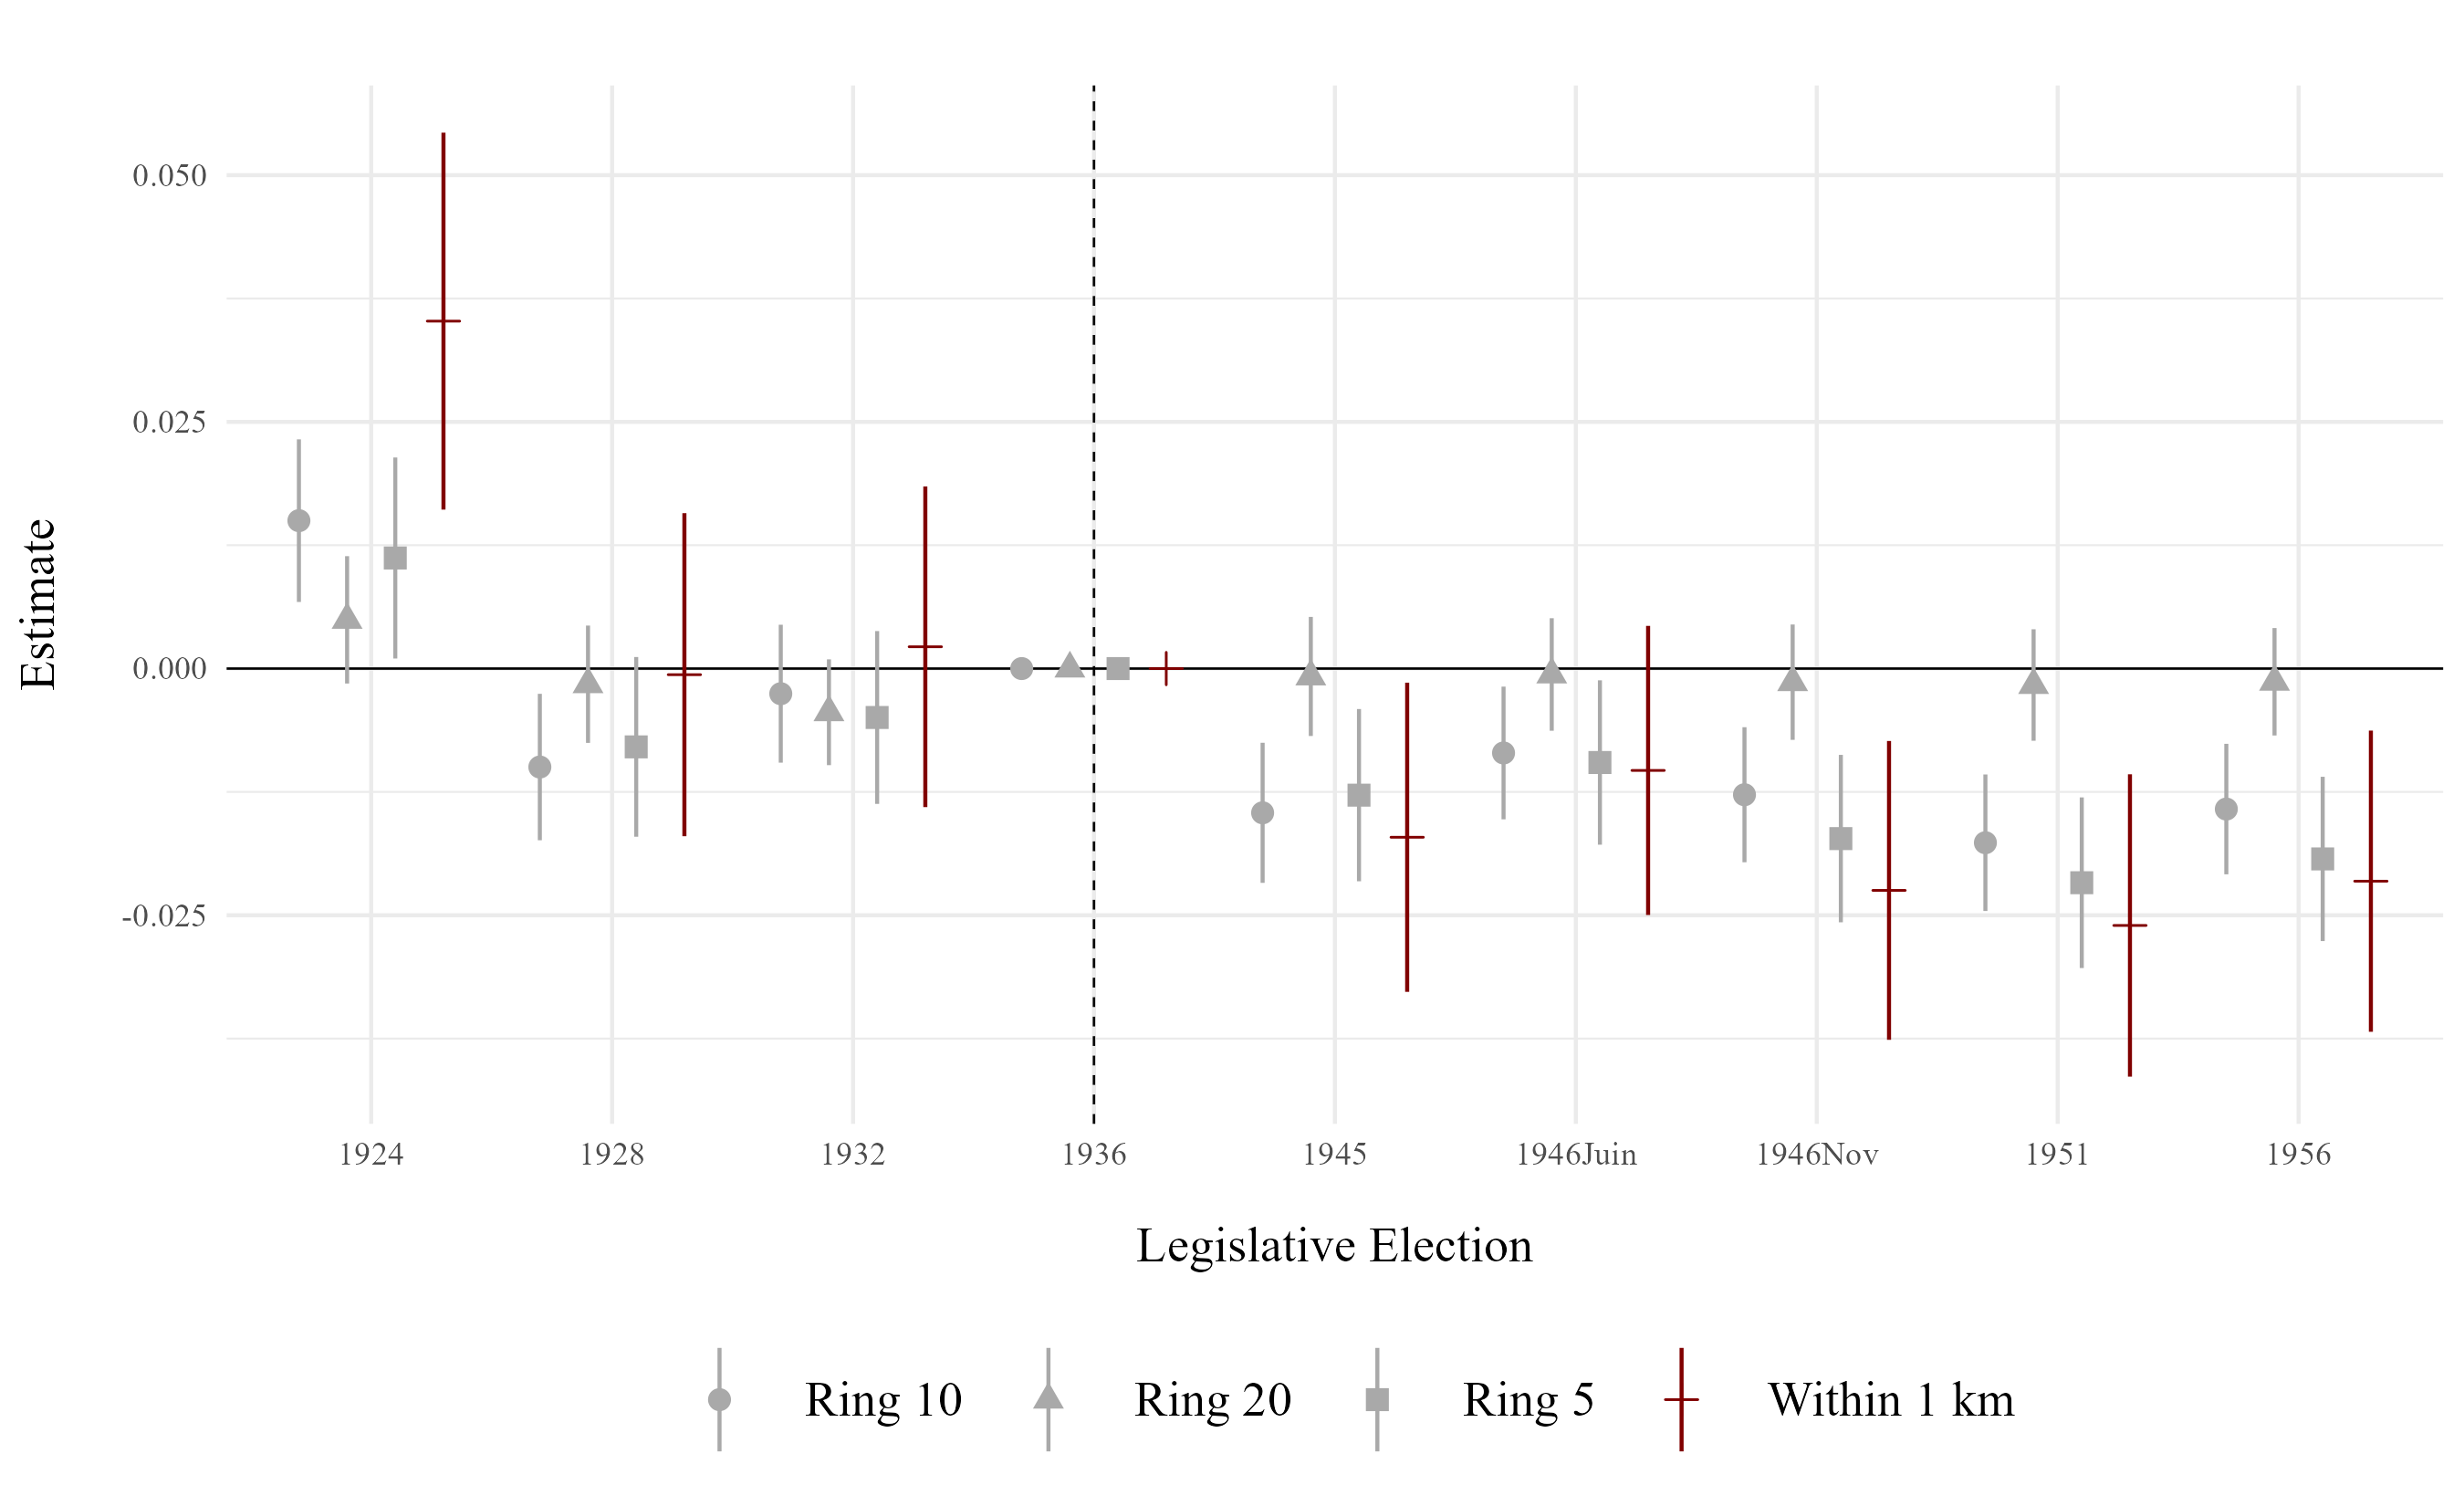
\includegraphics[width=0.8\linewidth]{../figures/results/political/pvoixSFIO_event_study.png}
  \label{fig:SFIO_all}
   \begin{minipage}{0.7\textwidth}
        \vspace{0.5em}
        {\footnotesize Notes: This graph reports the estimates from \cref{equation:political}, where the coefficient for each ring is estimated using municipalities located 20–40 km away as the control group. Error bars plot the interval confidence at 95\%. Standard errors are clustered at the municipality level.\par}
        \end{minipage}
\end{figure}


\begin{figure}[htbp]
  \centering
  \caption{Impact of refugee camps on communist vote shares - ring estimations}
  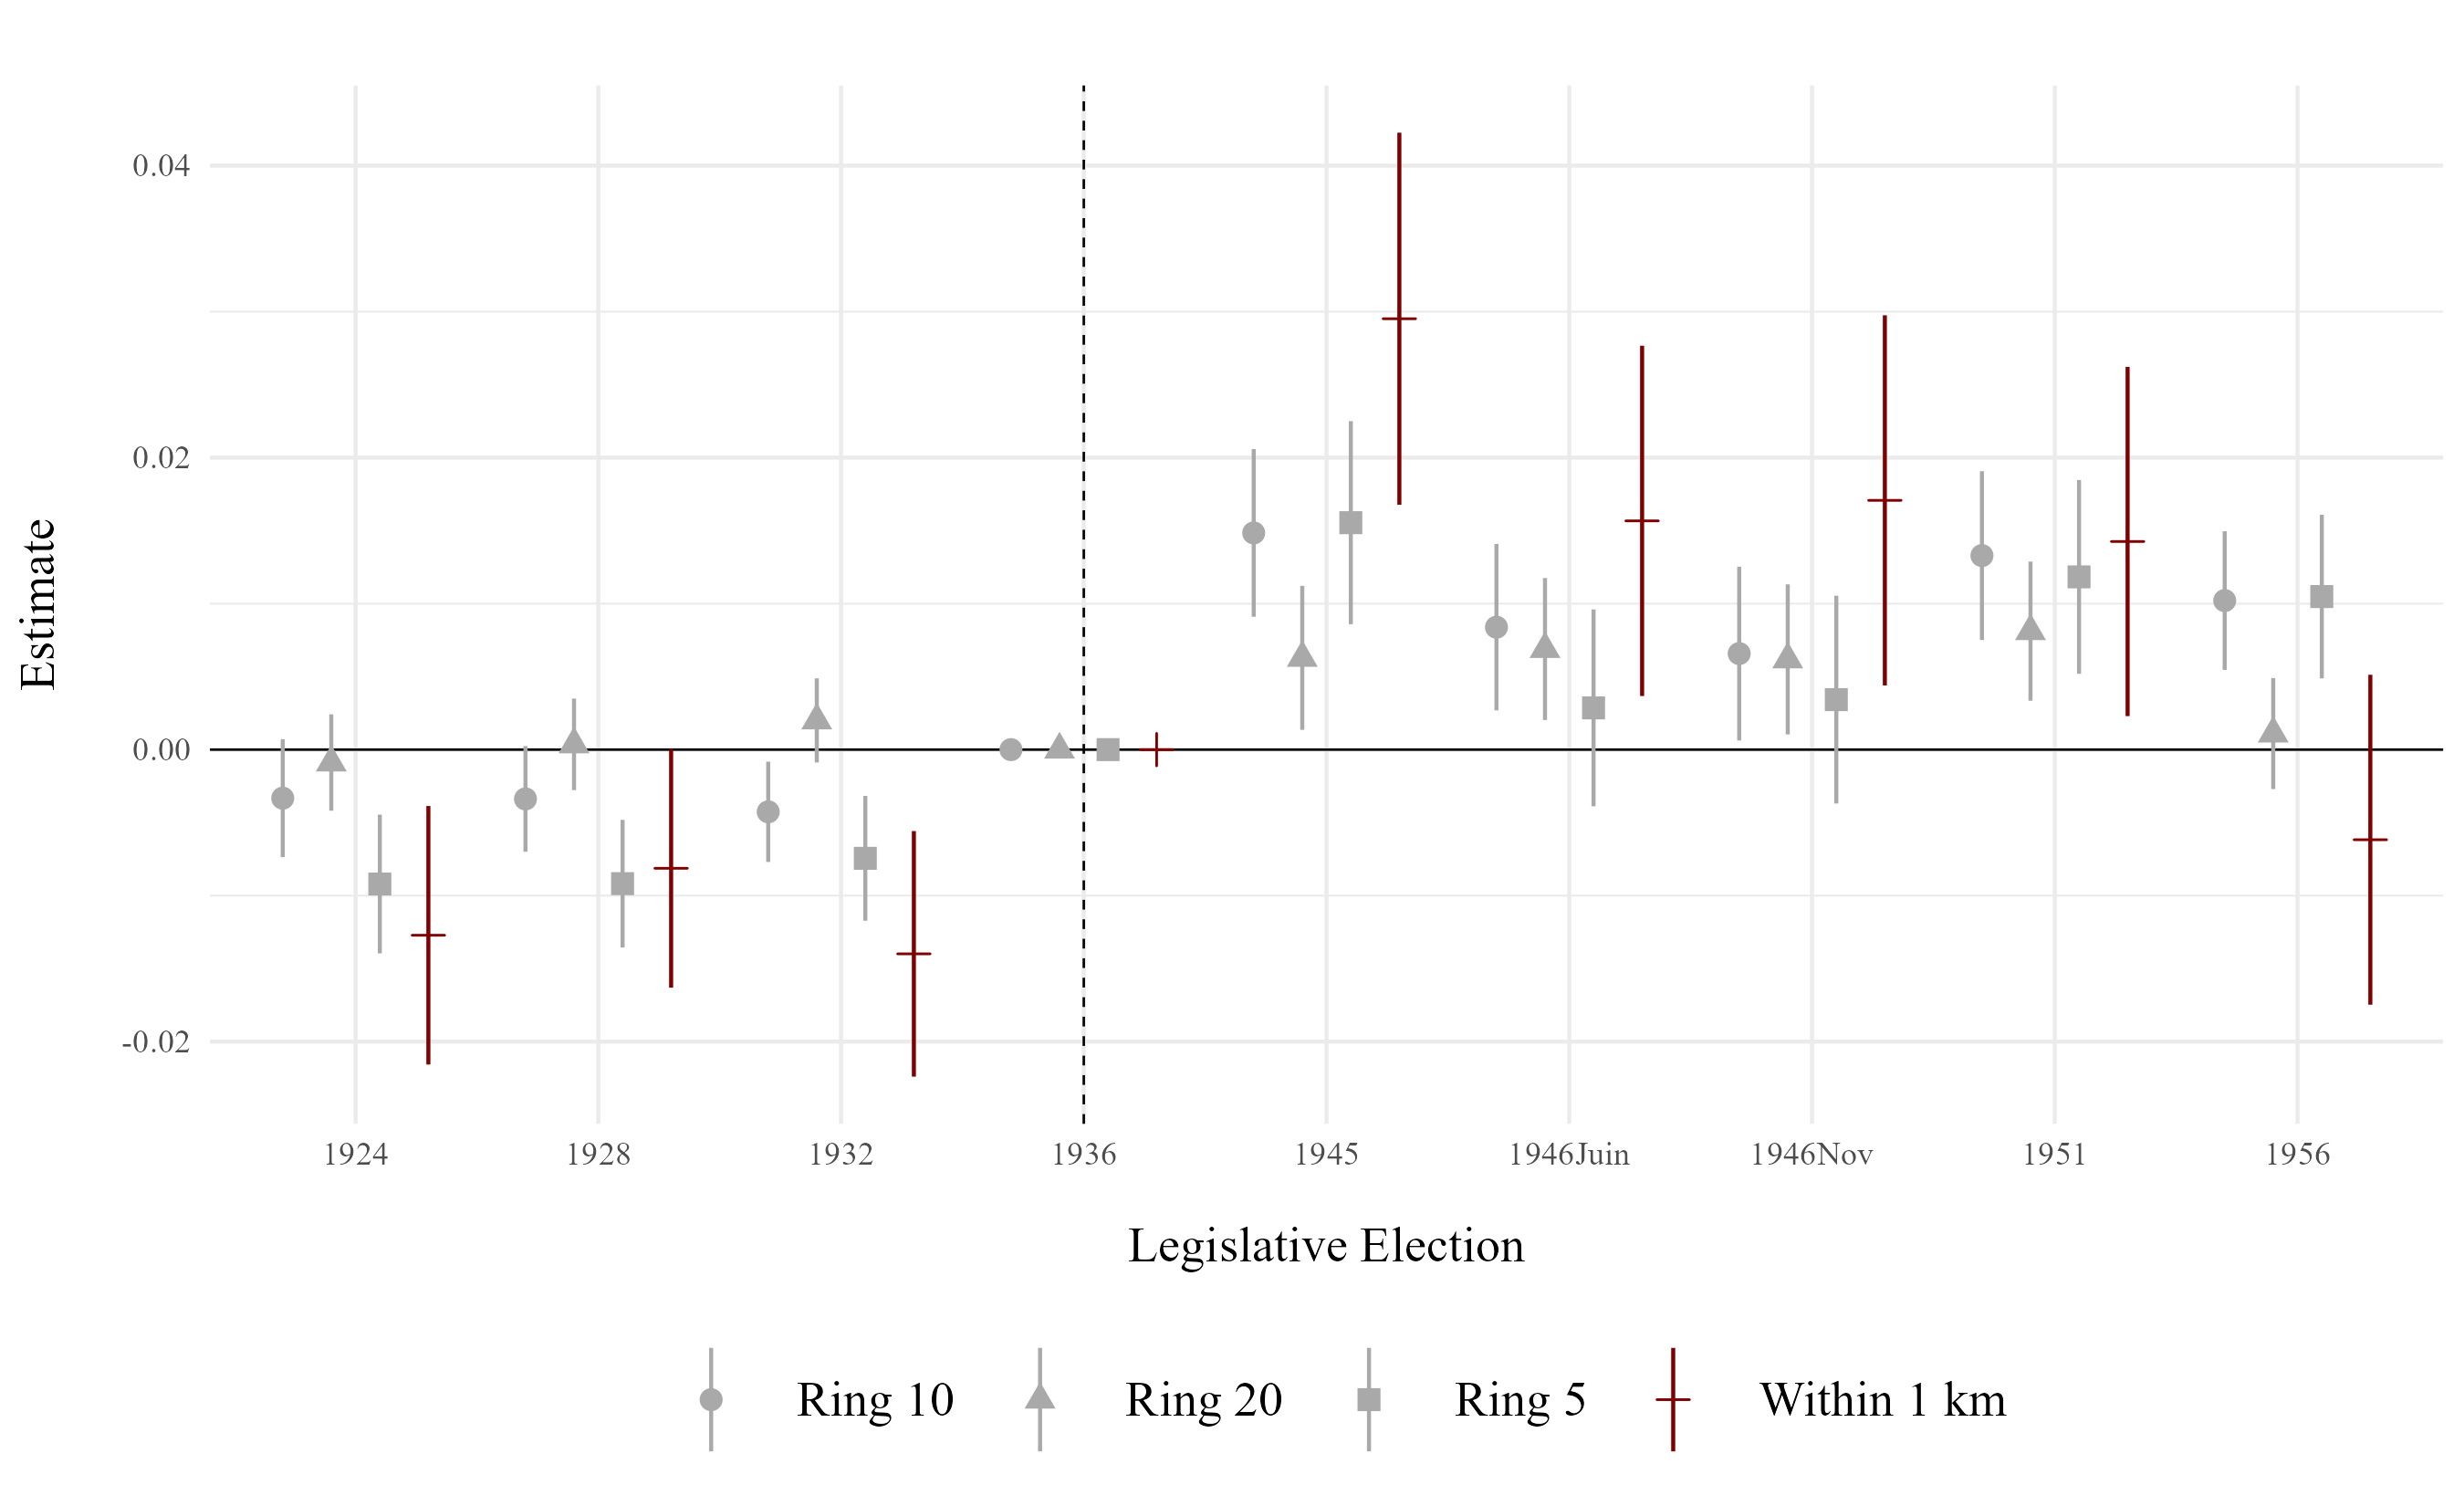
\includegraphics[width=0.8\linewidth]{../figures/results/political/pvoixPCF_event_study.png}
  \label{fig:PCF_all}
   \begin{minipage}{0.7\textwidth}
        \vspace{0.5em}
        {\footnotesize Notes: This graph reports the estimates from \cref{equation:political}, where the coefficient for each ring is estimated using municipalities located 20–40 km away as the control group. Error bars plot the interval confidence at 95\%. Standard errors are clustered at the municipality level.\par}
        \end{minipage}
\end{figure}

\begin{figure}[htbp]
  \centering
  \caption{Impact of refugee camps on the socialist vote share - by size}
  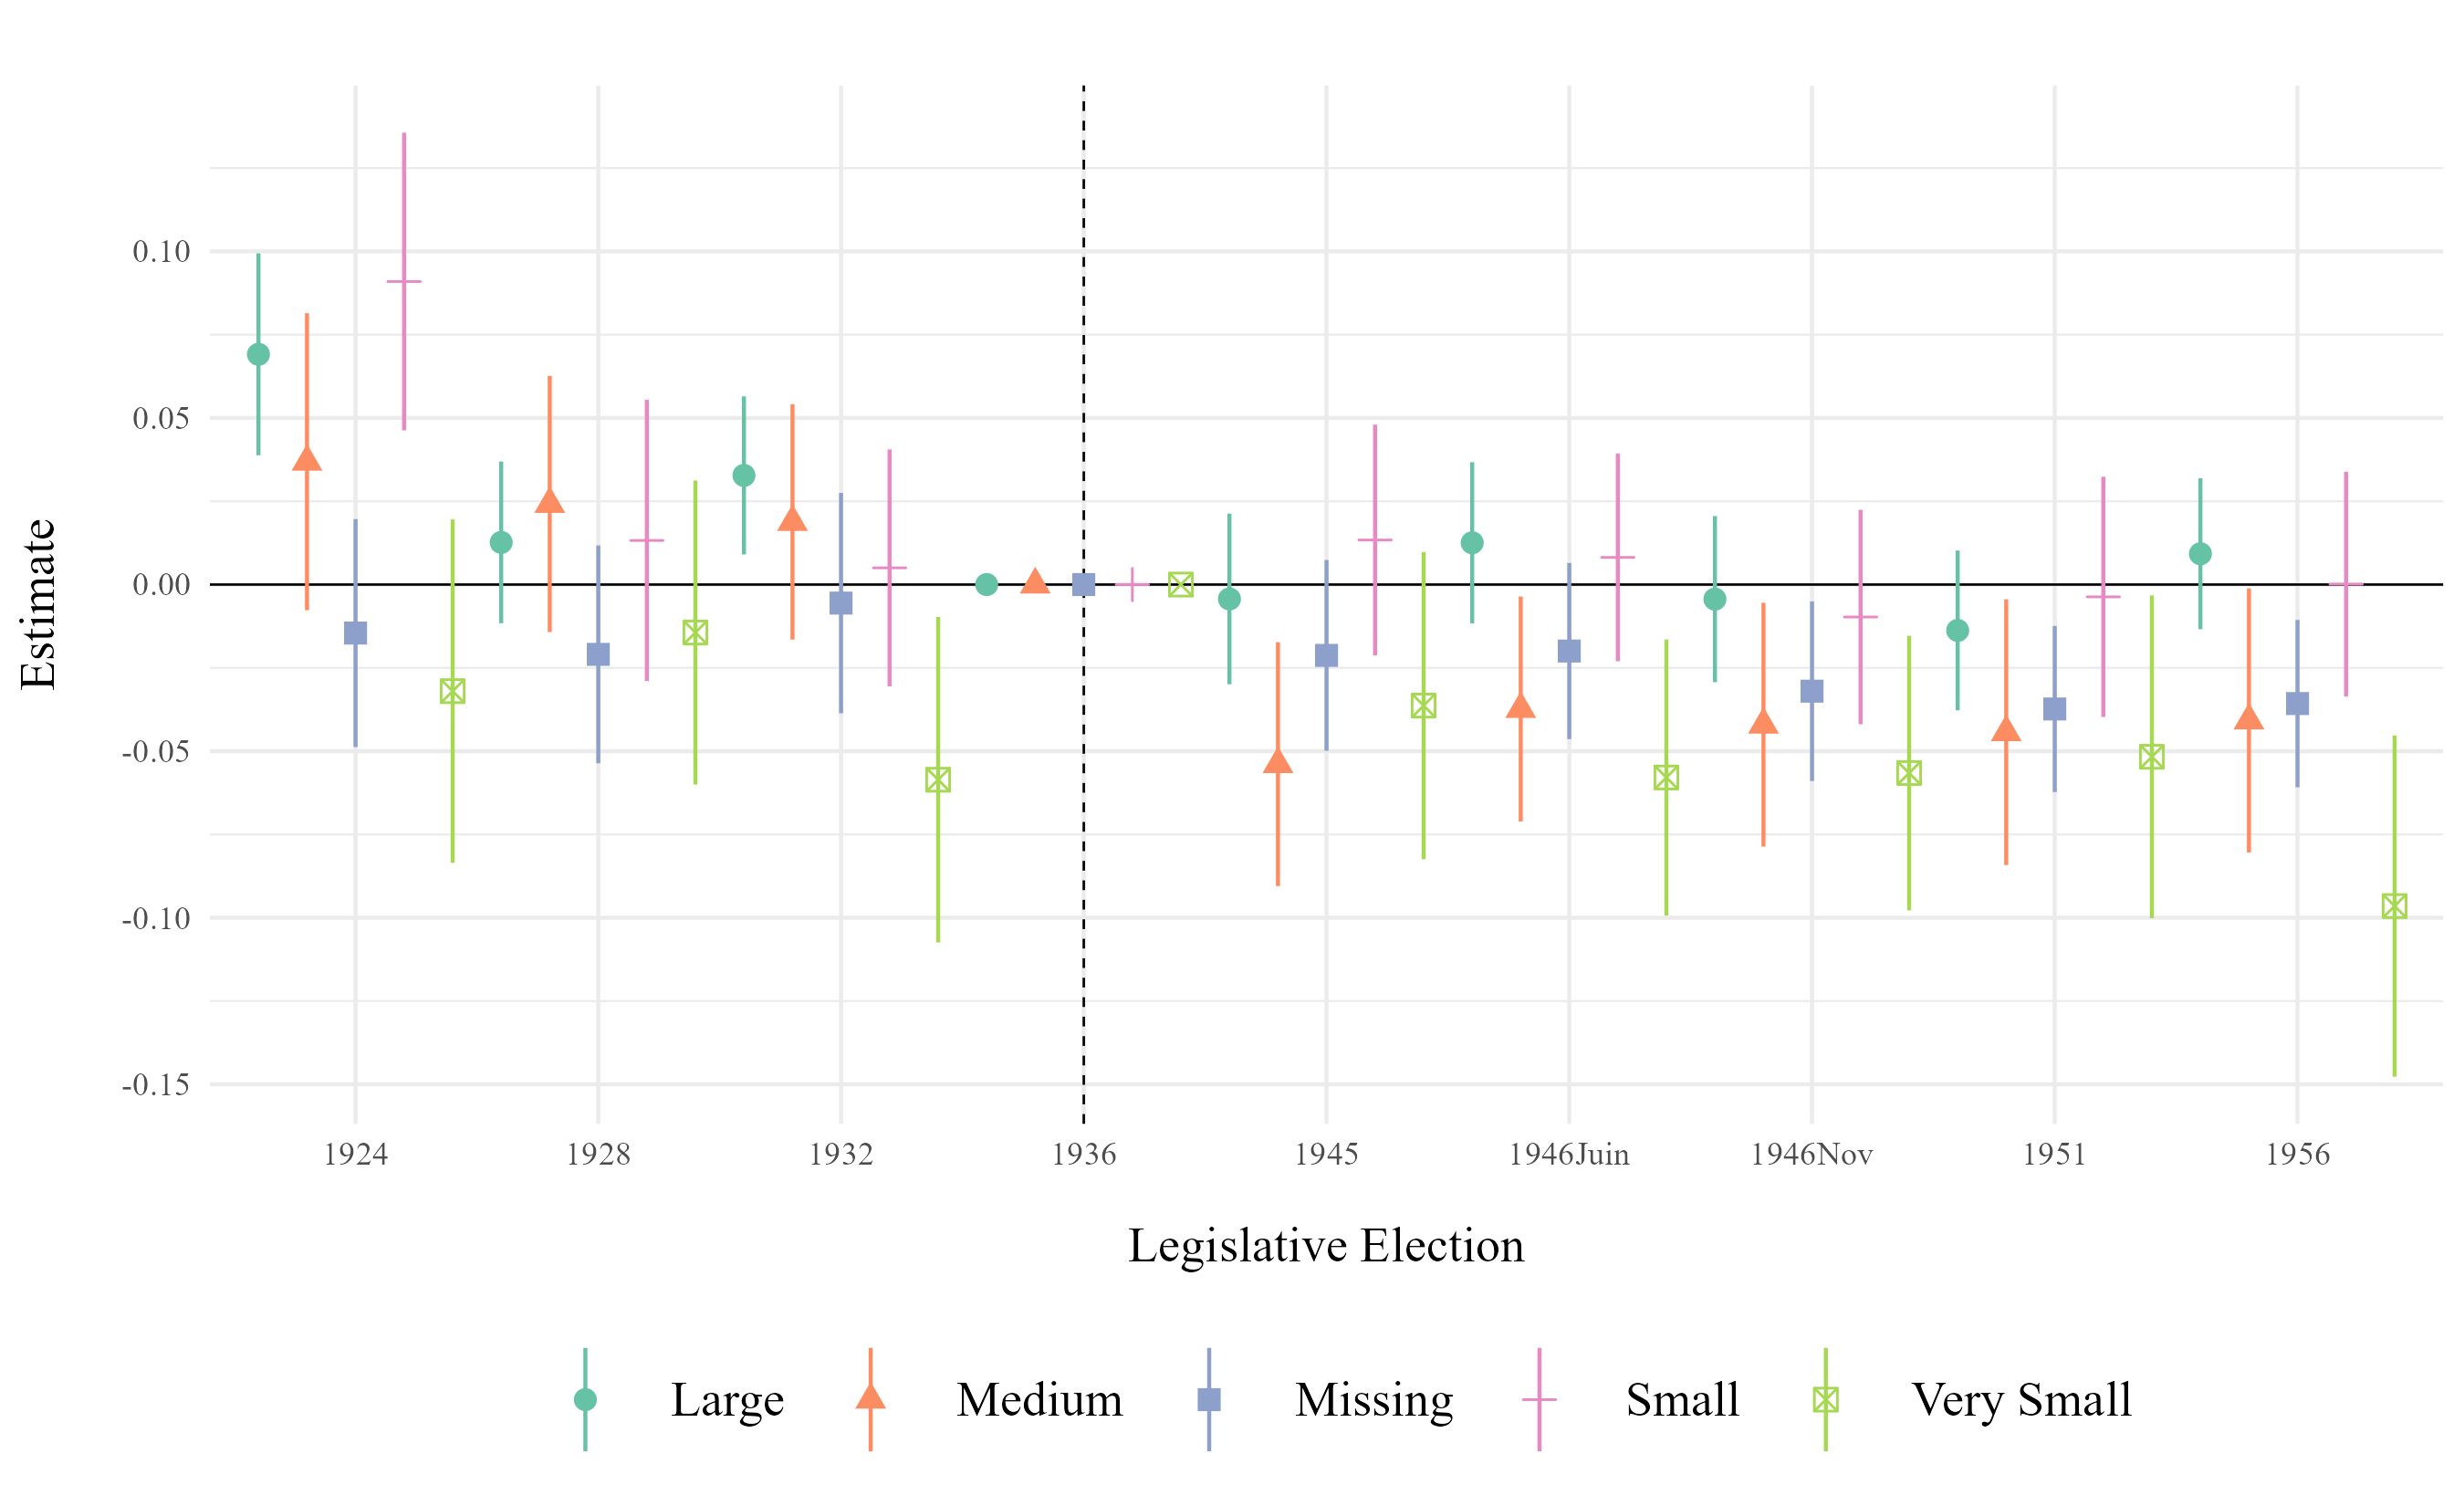
\includegraphics[width=0.8\linewidth]{../figures/results/political/sfio_size.png}
  \label{fig:SFIO_all}
   \begin{minipage}{0.7\textwidth}
        \vspace{0.5em}
        {\footnotesize Notes: This graph reports the estimated effect for each camp size, using as the control group municipalities without any other type of camp located 20–40 km away. Error bars plot the interval confidence at 95\%. Standard errors are clustered at the municipality level.\par}
        \end{minipage}
\end{figure}

\begin{figure}[htbp]
  \centering
  \caption{Impact of refugee camps on the communist vote share - by size}
  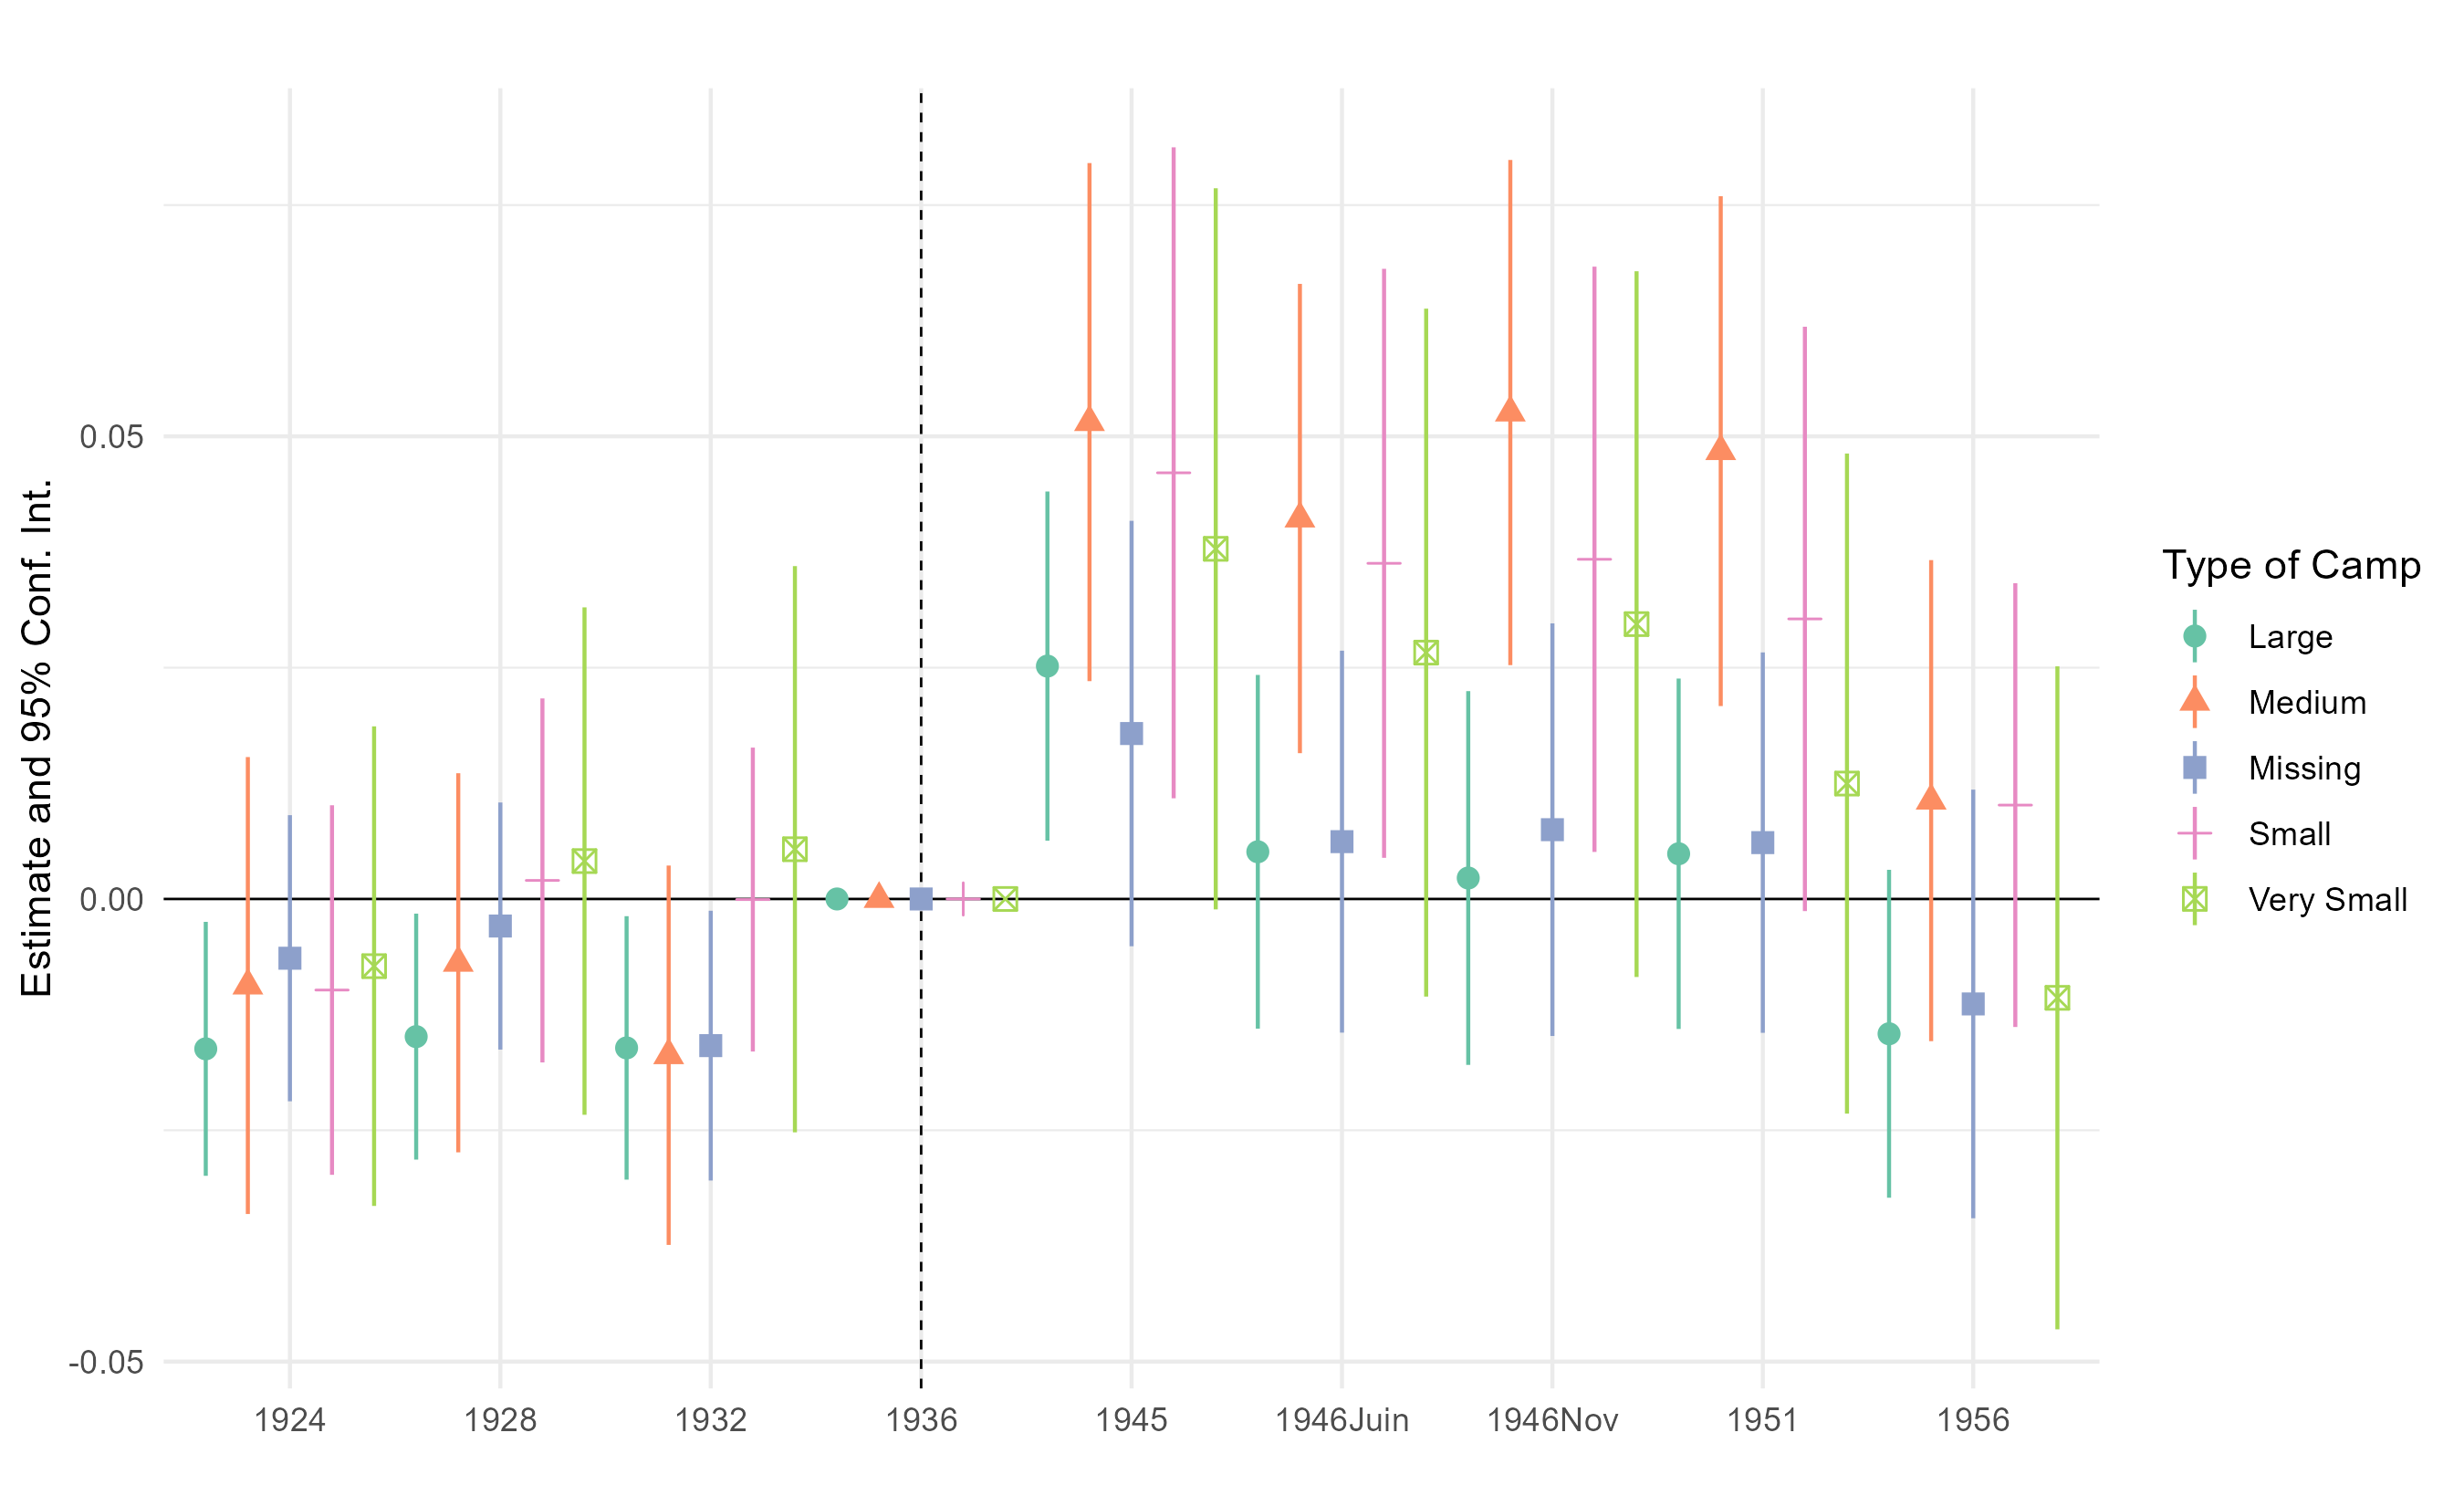
\includegraphics[width=0.8\linewidth]{../figures/results/political/communist_size.png}
  \label{fig:SFIO_all}
   \begin{minipage}{0.7\textwidth}
        \vspace{0.5em}
        {\footnotesize Notes: This graph reports the estimated effect for each camp size, using as the control group municipalities without any other type of camp located 20–40 km away. Error bars plot the interval confidence at 95\%. Standard errors are clustered at the municipality level.\par}
        \end{minipage}
\end{figure}

\begin{comment}

\clearpage
\section{Historical Context}


\subsection{The Arrival and Welcoming of the Refugees}

\subsubsection*{The Spanish Civil War and the Different Migrations Flows}

The large majority of the migrations flows from Spain, related with the Civil War, occur between 1936 and 1939. The timing of the migrations is directly related with the victories of the Nationalist groups over the Republicans. Dreyfus-Armand (2002) identifies three major waves of Spanish refugees to France between 1936 and 1939.
\begin{enumerate}
    \item The first one occurs in August 1936 and corresponds to the fall of the Republican force in the Basque Country. This wave is mainly composed of civilians, although soldiers also entered in French territory, mainly in order to reach Perpignan and then the Republican zone in Catalonia. Most of the refugees at this time are encouraged to come back to Spain. This wave represents around 15,000 refugees.
    \item The second wave occurs in 1937. The violence of the fighting between Republican and the Nationalists, especially the final assault against Bilbao, led the Republican authorities to evacuate the city. With the collaboration of the French authorities, more than 120,000 individuals, both soldiers and civilians.
    \item The last and biggest flow of refugees occurs in January 1939. This flow is known as ``La Retirada" (\textit{The Retreat}) and occurs after the Fall of Barcelona. This flow is both composed of soldiers but also civilians fleeing the intensive bombings. Most of the refugees cross the border by the Pyrenees, for instance in Le Perthus. Estimations of this amount of persons who cross the border differ. In March 1939, the French Assembly, through the Commission of Foreign Affairs, estimated that 450,000 refugees have crossed the border. At the same period, the French Ministry of Interior estimates that 300,000 soldiers and 214,000 civilians crossed the border. 
    \end{enumerate}

French Authorities, specially after 1938, initiate several policies in order to encourage the repatriation of refugees. For instance, at the end of 1938 and before the \textit{Retirada}, only 45,000 Spanish are still in France\footnote{from this number, a quarter are children according to J. Rubio, La Emigracion de la guerra civil de 1936-1939 (1982).}.

\subsubsection*{The Internment Camps}

Since the beginning of the Civil War, the guiding principle of the French Governments is to encourage repatriations of refugees. In a context of growing political tensions in Europe, the presence of thousands of refugees, some of who are politically very active, is considered as a major source of instability by the authorities. In Febuary 1939, France signed the Berard-Jordan Agreement with Franquist Spain, in order to facilitate the repatriation of refugees. As a consequence, between April 1rst 1939 (end of the Civil War) and the end of the year, thousands of refugees returned to Spain. During this time, the repatriation of refugees have been used several time by Franco to put pressure on the French Government, especially in order to push France to respect the terms of the agreement.
(for instance on the restitution of goods that had been transferred to France during the War). \\
In May-June 1939, evaluations estimates the number of refugees in France to be around 350,000 (including 155,000 civilians), and 250,000 in August of the same year\footnote{Archive du Ministère des Affaires Etrangères, série Europe 1918-1940), sous-série Espagne, vol. 189.}. At the end of 1939, French authorities estimated the number of refugees to be of 180,000 individuals (including 45,000 women and children)\footnote{Ibid.}. \\

The welcoming of refugees essentially considered as ``improvised", and refugees, both soldiers and families, are often put in old factories or closed down prison\footnote{Les camps sur la plage, un exil espagnol (avec Geneviève Dreyfus-Armand), Autrement, 1995}. Concentration camps are built for the first time in January 1939 when the largest amount of refugee starts to cross the border after the victories of Nationalists in Barcelona. 

\subsection{The Second World War and the Political Exile}

\subsubsection*{The Involvement during WWII}

\subsubsection*{The Post-War Exile until the Fall of Franco}

The exodus from Spain with the Civil War goes on after the Second World War and France Liberation. Estimations evaluate that around 10,000 immigrants from Spain have entered France each year between 1947 and 1949. 

\subsubsection*{The Political and Cultural Transmission}

\clearpage
\subsection{The Political Context in France}

\subsection*{Main parties during the interwar period}

The French Left during the interwar period was structured around three major political forces alongside several smaller organizations. The central pillars were the Radical-Socialists (RAD-SOC) —who, despite their name, occupied a space closer to liberal centrism—the Socialist Party (SFIO), and the Communist Party (PCF). Among the minor parties, the Republican Socialist Union held particular relevance, positioned ideologically between the Radicals and the Socialists, while a faction of dissident communists formed the Proletarian Union (Pickersgill, 1939)

In 1924, most of the left-wing parties (with the exception of the Communists) created an electoral alliance known as the Cartel des Gauches. This coalition achieved notable success in the legislative elections of 1924. Its cohesion weakened in 1928 and the the conservatives and moderates return to power under the leadership of Raymond Poincaré. The elections of 1932 once again give a majority to the Radicals and the Socialists. The Communists, however, remained outside of this arrangement until 1935, when the Third International urged communist parties across Europe to collaborate with democratic forces in the fight against fascism. This strategic shift laid the foundations of the Front Populaire, which brought together the full spectrum of left-wing parties (Pickersgill, 1939). Léon Blum, leader of the Socialist Party, becomes Prime Minister and his government implements a series of major social reforms as the introduction of the forty-hour work week \textcolor{red}{(Reference)}.

Following the classification of \cite{piketty_histoire_2023}, we divide the political forces present in the 1936 legislative elections in ten main forces. \textcolor{red}{(Reference)} for the explanation of the parties. 

\begin{description}
\item[Left-wing parties]: 
\begin{description}
    \item[PCF:] French Communist Party (Parti Communiste Français) and organizations close to the communists. Created in 1920 during the Tours Congress, when a majority of the SFIO decides to join the Third International (Comintern). At the time, it positions itself on the far left with a revolutionary and internationalist agenda. Its main leaders include Maurice Thorez and Jacques Duclos. 
    \item[SFIO:] Socialist party (Section Française de l’Internationale Ouvrière) and organizations close to the socialists. Created in 1905, it represents the Socialist movement. It adopts a Marxist orientation in theory but acts reformist in practice. Its most notable leaders are Léon Blum and Paul Faure.
    \item[RAD-SOC:] Candidates presented by the Radical Party (Parti Radical et Radical-Socialiste) and organizations close to the radicals. Founded iin 1901, the Radical and Radical-Socialist Party is France’s oldest political party. Influenced by Freemasonry, it championed civil liberties, anticlericalism, universal suffrage, and anti-colonialism. The party reached its peak in the interwar period under leaders like Édouard Herriot and Édouard Daladier. From the 1930s, while remaining anchored on the left (Cartel des gauches, Popular Front), it pursued moderate governance and came to embody “traditional” republican values—laïcité and free public education. During World War II, the party split between supporters of Pétain, resistance figures, and collaborators, suffering repression under Vichy. After Liberation, it was associated with the failed Third Republic and challenged by the MRP and SFIO. Attempts at modernization under Pierre Mendès France from 1955 exposed deep internal divisions, culminating in a right-wing split and the creation of the Centre républicain in 1956 francearchives_parti_radical \citep{francearchives_parti_radical}. 
    \item[DVG:] candidates presented by parties and organizations close to the communist or socialist movement (Proletarian Union, Communist Socialist Union, etc.).
    \item[USR:] candidates presented by the Republican Socialist Union and by related organizations (Independent Socialists, Independent Left, dissident Radical Party – Camille Pelletan, Young Republic, Frontist Party, etc.).

    \end{description}
\item[Right-wing parties]: 
\begin{description}
    \item[AD:] candidates presented by the Democratic Alliance and affiliated parties and organizations as Republican Left, Independent Radicals, Popular Democrats (Parti Démocrate Populaire), Independent Republicans, etc. Parti Démocrate Populaire (PDP) is founded in 1924, embodies Christian democratic and center-right values. One of its most important leaders is Auguste Champetier de Ribes. The PDP can be seen as the precursor to the postwar Mouvement Républicain Populaire (MRP).
    \item[FR-URD:] candidates presented by the Republican Federation (Fédération Républicaine) and the Republican and Democratic Union (as well as the National Republican Party). the Fédération Républicaine was founded in 1903 and defends conservative and pro-business interests. 
    \item[AGR:] candidates presented by various Agrarian and Peasant parties, Independent Agrarians, Agrarian Republicans, etc.
    \item[DVD:] miscellaneous right-wing candidates: Social Action Republicans, Independent Popular Action, Independent Social Action, Catholics, Conservatives.
\end{description}
\item [Others]: 
\begin{description}
    \item[DIV:] miscellaneous unclassifiable candidates (Regionalists, etc.).
    \end{description}
\end{description}

The interwar period in France is also characterized by the emergences of far-rights movements. The \textit{Action Française}, founded in 1899 by Charles Maurras, promotes monarchism and antisemitism. The Parti Social Français (PSF) emerges in 1936 out of the transformation of the veterans’ league Croix-de-Feu, following the dissolution of paramilitary leagues by the government of the Front Populaire. Under the leadership of Colonel François de La Rocque, the PSF becomes the first mass party of the French right, with hundreds of thousands of members across the country. It defends conservative, nationalist, and authoritarian values while rejecting both parliamentary instability and revolutionary extremes. The party was not formed by the time of the legislative elections in 1935 and the outbreak of the war prevented it from consolidating \textcolor{red}{(Reference)}. 

\subsection{The Non-Intervention Policy of the Front Populaire and the Spanish Refugees}

The experience of the \textit{Front Populaire} was relatively short-lived. Divisions within the government, economic difficulties, and rising international tensions gradually undermined cohesion among the left-wing parties. The refusal of the Communist Party to participate directly in government, combined with the eventual withdrawal of the Radicals, left the Socialists increasingly isolated. By 1938, under the mounting threat of war in Europe and with the Spanish Civil War polarizing public opinion, the \textit{Front Populaire} government collapsed.

The fall of the \textit{Front Populaire} was due in part to the government's response to the outbreak of the Spanish Civil War. The policy of non-intervention adopted by the French government was decided by the head of government, Léon Blum, in the summer of 1936. More broadly, historians characterize French policy towards the conflict in Spain as one of ``non-intervention.'' This policy was rapidly adopted by the French government in August 1936, and then by the British authorities, with the explicit aim of avoiding direct involvement in the conflict and preventing its spillover into France (\cite{monier_2016}). \\
In practice, however, the stance of the French government during the conflict, although officially restrictive, has led some historians to speak of a policy of ``soft non-intervention''\footnote{\textit{Non-intervention relâchée} in French.} (\cite{salmon_2024}). This expression captures the shifts in the French position with regard to the Spanish Civil War, from strict control of military supplies to periods during which weapons transiting through French territory (mainly from the Soviet Union) were effectively allowed to enter Spain. In this sense, the Blum government, while formally committed to non-intervention, at times turned a blind eye to arms trafficking in favour of the Republicans at the border.\\

The perceived position of the different left-wing parties towards the Spanish Civil War and the refugees, although all member of the same electoral coalition in 1936, is quite different. 

The Socialist from the SFIO are taken responsible from both the choice of the non-intervention since Léon Blum refused to provide direct military support to the Republican forces against Franco. The choice of non-intervention proved politically costly for the French government, particularly for the SFIO and Léon Blum, who publicly assumed full responsibility for this decision. \cite{thiebaut_2008} argues that, in public opinion, this choice remained ``a legacy difficult to assume'' for the \textit{Front Populaire} and continued to ``poison the collective memory,'' especially among those who saw themselves as ``close to the socialist movement.'' \\ 

The position of the Radicals, are the less incline to both get involved into the conflict and to welcome the refugees. Although personally inclined, like the communists, to support military intervention in favour of the Republican forces, Blum ultimately accepted non-intervention in order to preserve the support of the Radicals and maintain the fragile coalition. After the end of the \textit{Front Populaire}, Edouard Daladier (RAD-SOC) became the head of the government with the support of the right-wing parties in 1938. They kept on the line that they were already defending at the time of the \textit{Front Populaire}, advocating for the minimal intervention into the conflict. The strict policy chosen by the Radicals towards the refugees during the \textit{Retirada}, are often seen as a concession made to the numerous xenophobic stereotypes of the public opinion \cite{laborie_2008}. It has to be noted, that the competition between the left-wing forces is fierce, especially in the South of France with regards to the issue of the Spanish Civil war. The Radicals, afraid of the arise of the SFIO and the Communists, were willing to be seen as the ``party of the order", against the willingness of the Communist to get more involved in the conflict. In 1939 for instance, the radical press largely paid tribute the the welcoming policies of the Daladier government, while the communist one soon characterized the refugees installations as ``concentration camps"  \cite{nicolas_2009}.

The French Communist party on the contrary to the two other components of the \textit{Front Populaire}, led a broad campaign advocating French intervention, played an active role in organizing the reception of Republican refugees in France, and saw thousands of communist militants enlist in the International Brigades to fight in Spain \cite{monier_2016}.



\subsection*{The political landscape after the Second World War}

Compared to the legislative elections of 1936, the PCF, SFIO, and RAD-SOC remained present in the political landscape, while other parties underwent certain transformations or newly emerged \cite{piketty_histoire_2023}.

\begin{description}
\item[Left-wing parties]: 
\begin{description}
    \item[DVG:] the classification refers now to new parties close to the communist or socialist movement, as the Parti Communiste Internationaliste, Union Progressiste, Trotskystes, socialistes hors SFIO, etc.
    \item [UDSR:] candidates presented by the Democratic and Socialist Union of the Resistance (Union Démocratique et Socialiste de la Résistance) and other independent organizations emerging from the Resistance.
    \item [AUG:] Candidates presented by various parties and organizations of the non-communist ‘other left’ (Trotskyists, Internationalist Communists, etc.
    \end{description}
\item[Right-wing parties]: 
\begin{description}
    \item [MRP]: candidates presented by the Popular Republican Movement (Mouvement Républicain Populaire) and affiliated organizations. In November 1944, left-wing Christian members of the Resistance founded the Mouvement Républicain Populaire (MRP). Paradoxically, however, its electorate leaned more to the right, a trend confirmed in the 1951 elections, when the party lost a significant share of its voters to the Rassemblement du Peuple Français (RPF), the Gaullist party created in 1947. The MRP eventually dissolved in 1966, giving way to the Centre Démocrate.
    \item [ADPAYS]: lists presented by various moderate right-wing candidates (former members of the pre-war Democratic Alliance (Alliance Démocratique), independent republicans, independents and peasants, etc.).
    \item [URDDVD]: lists presented by various right-wing candidates (former members of the pre-war Republican and Democratic Union (Union Républicaine et Démocratique) or Republican Entente (Entente Républicaine), as well as other conservative right-wing candidates).
    \item [PRL]: candidates presented by the Republican Party of Liberty (Parti Républicain de la Liberté) and affiliated organizations.
    \item [REP]: various lists of Republican Concentration, Republican Defense, and Republican Union. 
\end{description}
\end{description}

%Considering Cagé et al. 2023 PCF should have much more in 1936 (8 or 4 depending on what round we are considering)
\begin{table}[htbp]
  \centering
  \caption{Mean vote shares by party and year}
  \label{tab:means_votes}

  % latex table generated in R 4.5.0 by xtable 1.8-4 package
% Fri Mar  6 12:27:33 2026
\begin{tabular}{llllllllll}
  \toprule
Party & 1924 & 1928 & 1932 & 1936 & 1945 & 1946Juin & 1946Nov & 1951 & 1956 \\ 
  \midrule
SFIO & 28.84 & 17.62 & 21.06 & 20.46 & 21.28 & 21.37 & 18.57 & 14.32 & 15.90 \\ 
  PCF & 9.74 & 10.77 & 8.11 & 14.31 & 25.74 & 25.74 & 27.99 & 25.89 & 25.08 \\ 
  MRP & -- & -- & -- & -- & 23.62 & 28.83 & 26.72 & 13.67 & 11.16 \\ 
  RADSOC & 10.38 & 23.56 & 19.86 & 15.28 & 6.75 & 1.87 & 0.70 & 2.61 & 9.42 \\ 
  ADPAYS & -- & -- & -- & -- & 4.61 & -- & -- & -- & -- \\ 
  DVD & -- & 2.01 & 0.80 & 2.83 & 3.28 & 3.52 & 4.84 & 0.86 & 2.20 \\ 
  PRL & -- & -- & -- & -- & 2.23 & 7.09 & 2.81 & -- & -- \\ 
  RG & 13.91 & -- & -- & -- & 0.48 & -- & -- & -- & -- \\ 
  FRURD & -- & 21.33 & 10.91 & 12.78 & -- & -- & -- & -- & -- \\ 
  URERD & 30.78 & -- & -- & -- & -- & -- & -- & -- & -- \\ 
  ADRG & -- & 16.36 & 14.77 & -- & -- & -- & -- & -- & -- \\ 
  AD & -- & -- & -- & 24.29 & -- & -- & -- & -- & -- \\ 
  RGR & -- & -- & -- & -- & -- & 8.30 & 8.57 & 4.04 & 0.77 \\ 
  UIPRN & -- & -- & -- & -- & -- & -- & -- & 8.06 & -- \\ 
  RPF & -- & -- & -- & -- & -- & -- & -- & 21.36 & -- \\ 
  CNI & -- & -- & -- & -- & -- & -- & -- & -- & 13.98 \\ 
  UFFUDCA & -- & -- & -- & -- & -- & -- & -- & -- & 11.72 \\ 
   \bottomrule
\end{tabular}


  \vspace{0.5em}

  \begin{minipage}{0.9\textwidth}
    \footnotesize
    \textit{Note:} A dash (--) indicates that the party did not run in that election. Political labels follow \citet{piketty_histoire_2023}: SFIO – French Section of the Workers’ International (socialist), RAD SOC – Radical and Radical-Socialist Party, DIV – Various independents or unaffiliated candidates, FR URD – Republican Federation / Republican and Democratic Union (conservative right), DVG – Miscellaneous left (non-SFIO left), PCF – French Communist Party, DVD – Miscellaneous right (independent right), AGR – Agrarian or peasant lists, USR – Republican Socialist Union, AD – Democratic Alliance (republican right). \textit{Source:} \cite{piketty_histoire_2023}.
  \end{minipage}

\end{table}


\end{comment}




